% The generic method: prove that an implementation refines its spec through Aeneas.
% Context for the per-track decks, for example ../x25519-full-refinement.
% Build: latexmk -lualatex slides.tex
\documentclass[aspectratio=169,11pt]{beamer}

\usepackage{fontspec}
\setsansfont{DejaVu Sans}
\directlua{
  luaotfload.add_fallback("leanfallback", {"NotoSansMath:mode=harf;", "STIX Two Math:mode=harf;"})
}
\setmonofont{DejaVu Sans Mono}[Scale=0.9, RawFeature={fallback=leanfallback}]

\usepackage{tikz}
\usetikzlibrary{arrows.meta, positioning, calc, fit, backgrounds, shapes.misc, decorations.pathreplacing}

% Colors. Spec side, impl side, proof, trusted, gap. Same as the track decks.
\definecolor{refc}{HTML}{2B6CB0}
\definecolor{realc}{HTML}{C05621}
\definecolor{proofc}{HTML}{2F855A}
\definecolor{trustc}{HTML}{718096}
\definecolor{gapc}{HTML}{C53030}
\definecolor{ink}{HTML}{1A202C}
\definecolor{paper}{HTML}{FFFFFF}

\setbeamercolor{normal text}{fg=ink, bg=paper}
\setbeamercolor{frametitle}{fg=ink}
\setbeamercolor{title}{fg=ink}
\setbeamercolor{structure}{fg=refc}
\setbeamerfont{frametitle}{size=\Large, series=\bfseries}
\setbeamertemplate{navigation symbols}{}
\setbeamertemplate{footline}{%
  \hfill\textcolor{trustc}{\scriptsize\insertframenumber/\inserttotalframenumber}\hspace{1.2em}\vspace{0.8em}}

\tikzset{
  >={Stealth[length=2.4mm]},
  box/.style={draw, rounded corners=3pt, thick, align=center, inner sep=5pt, font=\small},
  spec/.style={box, draw=refc, fill=refc!8},
  impl/.style={box, draw=realc, fill=realc!8},
  proof/.style={box, draw=proofc, fill=proofc!10},
  trust/.style={box, draw=trustc, fill=trustc!10},
  gap/.style={box, draw=gapc, fill=gapc!6, dashed},
  tool/.style={box, draw=ink!60, fill=ink!4},
  doc/.style={box, draw=ink!60, fill=paper, double, double distance=1pt},
  flow/.style={->, thick, ink!70},
  proved/.style={<->, very thick, proofc},
  rel/.style={-, very thick, proofc, dashed},
  label/.style={font=\scriptsize, align=center},
}

\newcommand{\code}[1]{\texttt{#1}}
\newcommand{\specside}[1]{\textcolor{refc}{#1}}
\newcommand{\implside}[1]{\textcolor{realc}{#1}}
% Refinement: S \refines I reads "I refines S". Change here to switch the symbol.
\newcommand{\refines}{\sqsubseteq}

\title{Does the implementation compute what the spec computes?}
\subtitle{A method to prove refinement between two Rust programs in Lean, through Aeneas}
\author{ref-impl-simulation}
\date{November 2026}

\begin{document}

% ---------------------------------------------------------------- 1
\begin{frame}
  \titlepage
  \centering
  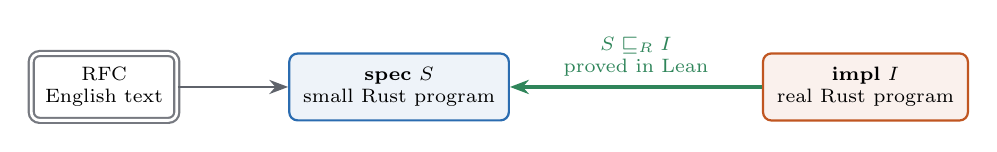
\begin{tikzpicture}
    \node[doc, font=\scriptsize] (rfc) {RFC\\English text};
    \node[spec, font=\scriptsize, right=1.4cm of rfc] (s) {\textbf{spec} $S$\\small Rust program};
    \node[impl, font=\scriptsize, right=3.2cm of s] (i) {\textbf{impl} $I$\\real Rust program};
    \draw[flow] (rfc) -- (s);
    \draw[proved, ->] (i) -- node[above, label, text=proofc] {$S \refines_R I$\\proved in Lean} (s);
  \end{tikzpicture}
\end{frame}

% ---------------------------------------------------------------- 2
\begin{frame}[t]{Two Rust programs for one RFC}
  \vspace{0.9em}
  \centering
  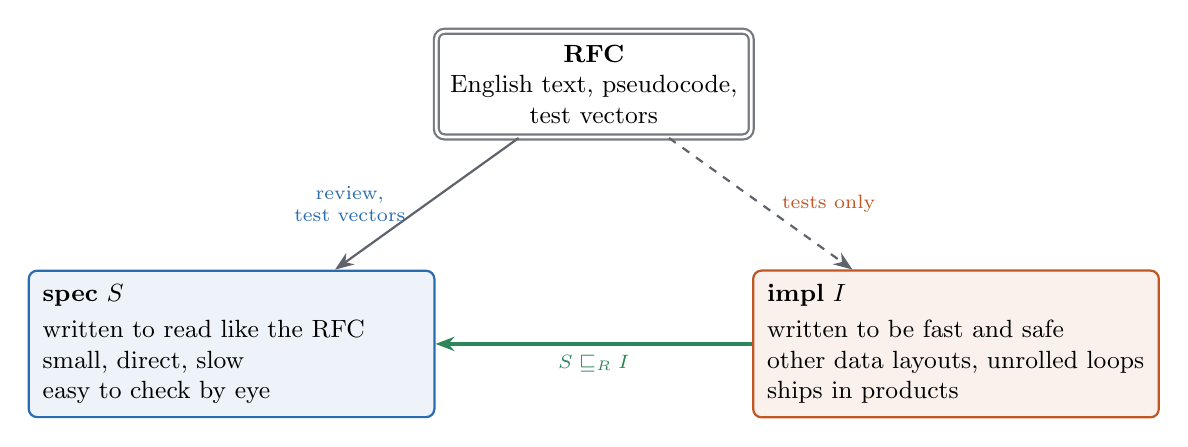
\begin{tikzpicture}[every node/.append style={font=\scriptsize}]
    \node[doc, minimum width=3cm] (rfc) at (0, 0.5) {\textbf{RFC}\\English text, pseudocode,\\test vectors};
    \node[spec, text width=4.8cm, align=flush left] (s) at (-4.6, -2.8)
      {\textbf{spec} $S$\\[2pt]
       written to read like the RFC\\
       small, direct, slow\\
       easy to check by eye};
    \node[impl, text width=4.8cm, align=flush left] (i) at (4.6, -2.8)
      {\textbf{impl} $I$\\[2pt]
       written to be fast and safe\\
       other data layouts, unrolled loops\\
       ships in products};
    \draw[flow] (rfc) -- node[left=4pt, label, text=refc, pos=0.5] {review,\\test vectors} (s);
    \draw[flow, dashed] (rfc) -- node[right=4pt, label, text=realc, pos=0.5] {tests only} (i);
    \draw[proved, ->] (i) -- node[below, label, text=proofc] {$S \refines_R I$} (s);
  \end{tikzpicture}
  \vspace{-0.6em}

  \begin{itemize}\footnotesize
    \item People can read $S$ and compare it with the RFC.
    \item It is more difficult to do the same for $I$.
    \item A proof that $I$ computes what $S$ computes moves the trust from $S$ to $I$.
    \item We write $S \refines_R I$: $I$ refines $S$ under a relation $R$.
  \end{itemize}
\end{frame}

% ---------------------------------------------------------------- 2b
\begin{frame}[t]{We do not start from zero: hacspec}
  \vspace{0.9em}
  \centering
  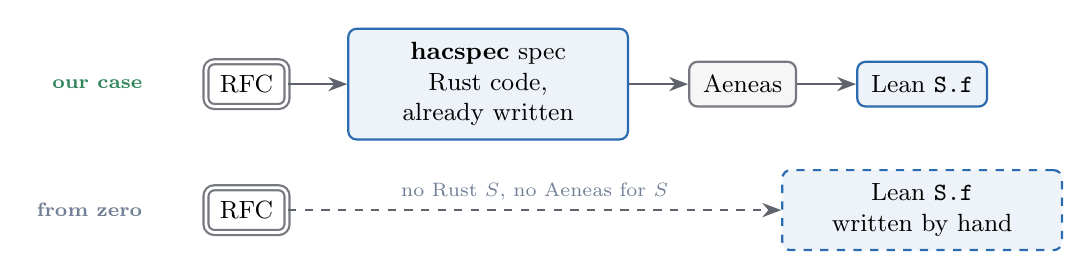
\begin{tikzpicture}[every node/.append style={font=\scriptsize}]
    \node[label, anchor=east, text=proofc] at (-0.4, 0) {\textbf{our case}};
    \node[doc] (rfc1) at (0.8, 0) {RFC};
    \node[spec, right=0.75cm of rfc1, text width=3.2cm] (hs) {\textbf{hacspec} spec\\Rust code,\\already written};
    \node[tool, right=0.75cm of hs] (ae) {Aeneas};
    \node[spec, right=0.75cm of ae] (ls1) {Lean \code{S.f}};
    \draw[flow] (rfc1) -- (hs);
    \draw[flow] (hs) -- (ae);
    \draw[flow] (ae) -- (ls1);

    \node[label, anchor=east, text=trustc] at (-0.4, -1.6) {\textbf{from zero}};
    \node[doc] (rfc2) at (0.8, -1.6) {RFC};
    \node[spec, dashed, text width=3.2cm] (ls2) at (ls1 |- rfc2) {Lean \code{S.f}\\written by hand};
    \draw[flow, dashed] (rfc2) -- node[above, label, text=trustc] {no Rust $S$, no Aeneas for $S$} (ls2);
  \end{tikzpicture}
  \vspace{0.8em}

  \begin{itemize}\footnotesize
    \item hacspec, and the language of the hax toolchain, are subsets of Rust for executable specs.
    \item So $S$ exists before we start. We reuse it and run Aeneas on it, as on $I$.
    \item Its fit to the RFC is trusted, and test vectors check it. A spec modelled on
      the real code (Ristretto follows dalek) cannot find an error that both share.
    \item Without such a spec, we can write $S$ directly in Lean and skip Aeneas for $S$.
    \item The price: old hacspec does not go through Aeneas as is.
      It needs a port or a shim, and both are trusted.
  \end{itemize}
\end{frame}

% ---------------------------------------------------------------- 3
\begin{frame}{The pipeline}
  \centering
  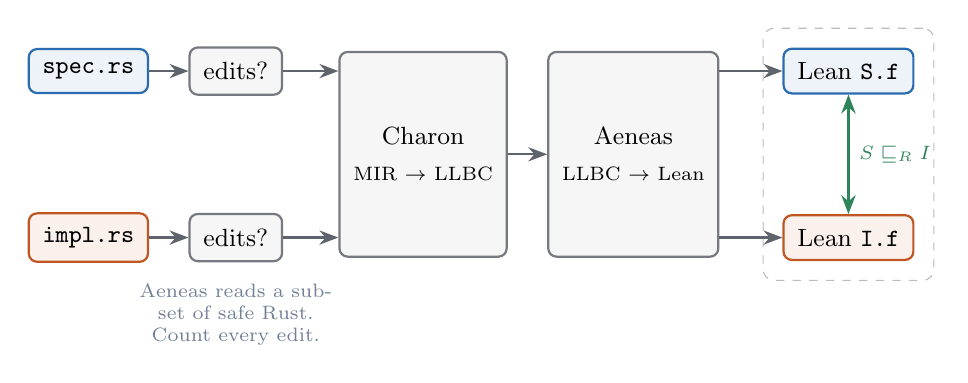
\begin{tikzpicture}[node distance=0.5cm and 0.5cm, every node/.append style={font=\scriptsize}]
    \node[spec] (srs) {\code{spec.rs}};
    \node[impl, below=1.5cm of srs] (irs) {\code{impl.rs}};
    \node[tool, anchor=west, minimum height=0.6cm] (es) at ($(srs.east)+(0.5,0)$) {edits?};
    \node[tool, anchor=west, minimum height=0.6cm] (ei) at ($(irs.east)+(0.5,0)$) {edits?};
    \node[tool, minimum height=2.6cm, anchor=west] (ch) at ($(es.east)!0.5!(ei.east)+(0.7,0)$)
      {Charon\\[2pt]\scriptsize MIR $\to$ LLBC};
    \node[tool, minimum height=2.6cm, right=0.5cm of ch] (ae) {Aeneas\\[2pt]\scriptsize LLBC $\to$ Lean};
    \node[spec, anchor=west] (ls) at ($(ae.east |- srs)+(0.8,0)$) {Lean \code{S.f}};
    \node[impl] (li) at (ls |- irs) {Lean \code{I.f}};

    \draw[flow] (srs) -- (es);
    \draw[flow] (irs) -- (ei);
    \draw[flow] (es.east) -- (ch.west |- es.east);
    \draw[flow] (ei.east) -- (ch.west |- ei.east);
    \draw[flow] (ch) -- (ae);
    \draw[flow] (ae.east |- ls) -- (ls);
    \draw[flow] (ae.east |- li) -- (li);
    \draw[proved] (ls.south) -- node[right, label, text=proofc] {$S \refines_R I$} (li.north);
    \begin{scope}[on background layer]
      \node[draw=ink!30, dashed, rounded corners, fit=(ls)(li), inner sep=7pt,
            label={[label]above:one Lake project}] {};
    \end{scope}
    \node[label, text=trustc, below=0.15cm of ei, text width=3cm]
      {Aeneas reads a subset of safe Rust. Count every edit.};
  \end{tikzpicture}
  \vspace{1.4em}

  \begin{itemize}\footnotesize
    \item Aeneas turns each Rust function into a pure Lean function in a \code{Result} monad.
    \item The question about 2 Rust programs becomes a question about 2 Lean functions.
  \end{itemize}
\end{frame}

% ---------------------------------------------------------------- 4
\begin{frame}[t,fragile]{The theorem $S \refines_R I$: a commuting square}
  \vspace{0.9em}
  \centering
  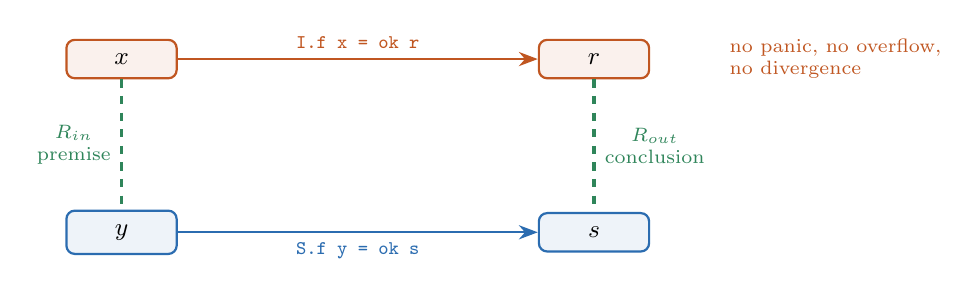
\begin{tikzpicture}
    \node[impl, minimum width=1.4cm] (x) at (0, 1.1) {$x$};
    \node[spec, minimum width=1.4cm] (y) at (0, -1.1) {$y$};
    \node[impl, minimum width=1.4cm] (r) at (6, 1.1) {$r$};
    \node[spec, minimum width=1.4cm] (s) at (6, -1.1) {$s$};
    \draw[flow, realc] (x) -- node[above, label, text=realc] {\code{I.f x = ok r}} (r);
    \draw[flow, refc] (y) -- node[below, label, text=refc] {\code{S.f y = ok s}} (s);
    \draw[rel] (x) -- node[left, label, text=proofc] {$R_{in}$\\premise} (y);
    \draw[rel] (r) -- node[right, label, text=proofc] {$R_{out}$\\conclusion} (s);
    \node[label, text=realc, anchor=west, align=left] at (7.6, 1.1)
      {no panic, no overflow,\\no divergence};
  \end{tikzpicture}
  \vspace{0.8em}

\begin{verbatim}
theorem I_refines_S (x : I.In) (y : S.In) (h : R_in x y) :
    I.f x ⦃ r => ∃ s, S.f y = .ok s ∧ R_out r s ⦄
\end{verbatim}
  \begin{itemize}\footnotesize
    \item $R = (R_{in}, R_{out})$.
    \item \code{⦃ ⦄} is the total-correctness triple of the Aeneas library.
    \item Both functions are deterministic, so the results agree whenever $R_{in}$ holds.
  \end{itemize}
\end{frame}

% ---------------------------------------------------------------- 5
\begin{frame}[t]{The relation maps $I$ data to $S$ data}
  \vspace{0.9em}
  \centering
  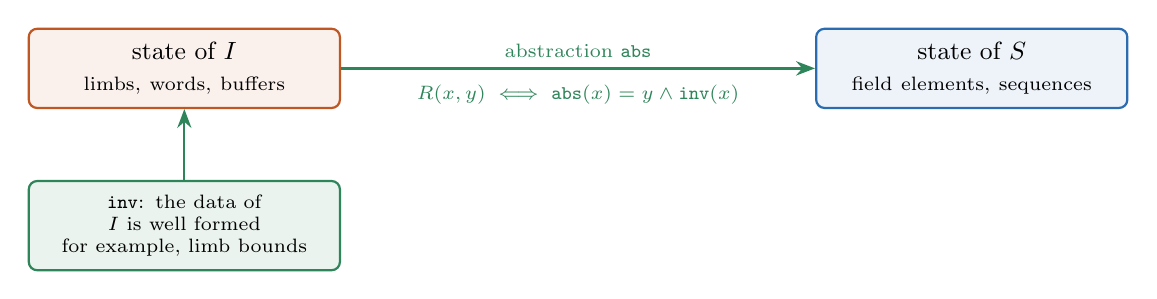
\begin{tikzpicture}
    \node[impl, text width=3.6cm] (id) at (0, 0) {state of $I$\\\scriptsize limbs, words, buffers};
    \node[spec, text width=3.6cm] (sd) at (10, 0) {state of $S$\\\scriptsize field elements, sequences};
    \draw[flow, very thick, proofc] (id) -- node[above, label, text=proofc] {abstraction \code{abs}}
      node[below=2pt, label, text=proofc] {$R(x, y) \iff \code{abs}(x) = y \wedge \code{inv}(x)$} (sd);
    \node[proof, below=0.9cm of id, text width=3.6cm, font=\scriptsize] (inv)
      {\code{inv}: the data of $I$ is well formed\\for example, limb bounds};
    \draw[flow, proofc] (inv) -- (id);
  \end{tikzpicture}
  \vspace{0.2em}

  \begin{columns}[T]
    \begin{column}{0.3\textwidth}\scriptsize
      \textbf{ChaCha20}\\
      equal lists of 32-bit words
    \end{column}
    \begin{column}{0.3\textwidth}\scriptsize
      \textbf{X25519}\\
      5 limbs of 51 bits map to \code{ZMod (2\textasciicircum255 - 19)}, limbs stay below $2^{52}$
    \end{column}
    \begin{column}{0.3\textwidth}\scriptsize
      \textbf{HPKE}\\
      equal byte strings, a map between algorithm identifiers
    \end{column}
  \end{columns}
  \vspace{0.4em}

  \begin{itemize}\footnotesize
    \item Each study defines its own relation.
    \item The invariant lets the next step start.
  \end{itemize}
\end{frame}

% ---------------------------------------------------------------- 6
\begin{frame}{The proof follows the call path}
  \centering
  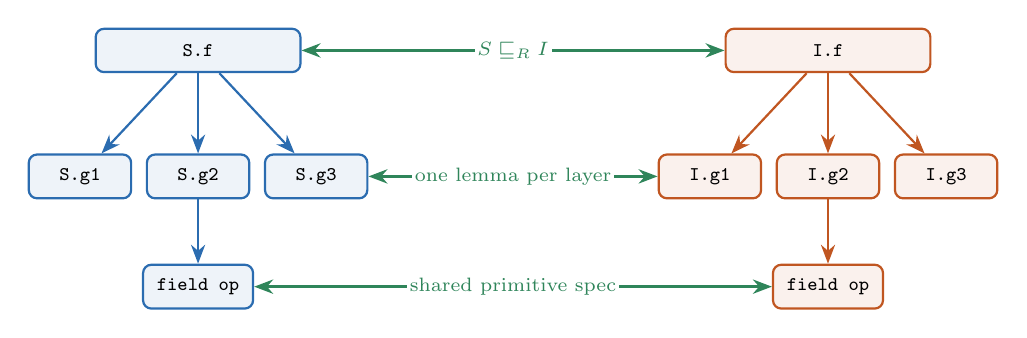
\begin{tikzpicture}[
      fn/.style={font=\scriptsize\ttfamily, minimum width=2.6cm, minimum height=0.55cm},
      lem/.style={label, text=proofc, fill=paper, inner sep=1pt}]
    \node[spec, fn] (s0) at (0, 0) {S.f};
    \node[impl, fn] (i0) at (8, 0) {I.f};
    \draw[proved] (s0) -- node[lem] {$S \refines_R I$} (i0);

    \foreach \k/\x in {1/-1.5, 2/0, 3/1.5} {
      \node[spec, fn, minimum width=1.3cm] (s\k) at (\x, -1.6) {S.g\k};
      \draw[flow, refc] (s0) -- (s\k);
    }
    \foreach \k/\x in {1/6.5, 2/8, 3/9.5} {
      \node[impl, fn, minimum width=1.3cm] (i\k) at (\x, -1.6) {I.g\k};
      \draw[flow, realc] (i0) -- (i\k);
    }
    \draw[proved] (s3) -- node[lem] {one lemma per layer} (i1);
    \node[spec, fn, minimum width=1.3cm] (s4) at (0, -3.0) {field op};
    \node[impl, fn, minimum width=1.3cm] (i4) at (8, -3.0) {field op};
    \draw[flow, refc] (s2) -- (s4);
    \draw[flow, realc] (i2) -- (i4);
    \draw[proved] (s4) -- node[lem] {shared primitive spec} (i4);
  \end{tikzpicture}
  \vspace{1.6em}

  \begin{itemize}\footnotesize
    \item Split each side at its calls.
    \item Prove one lemma for each pair of calls that match.
    \item The main theorem composes the lemmas.
    \item The leaves are often shared primitives: a field operation, a hash, a byte copy.
  \end{itemize}
\end{frame}

% ---------------------------------------------------------------- 7
\begin{frame}{Lockstep where the control flows match}
  \centering
  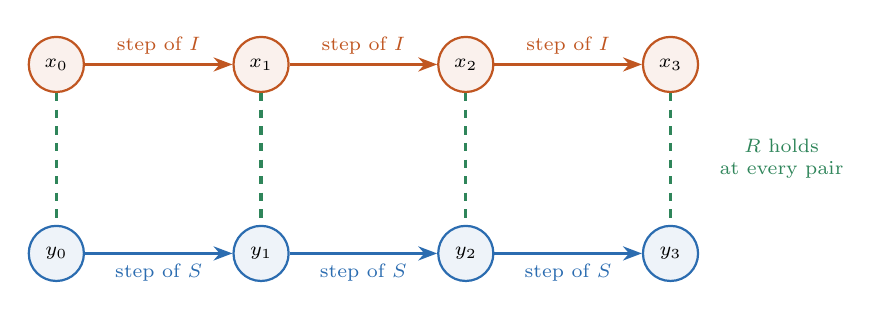
\begin{tikzpicture}[
      st/.style={draw, thick, circle, minimum size=0.7cm, inner sep=0pt, font=\scriptsize}]
    \foreach \k in {0,1,2,3} {
      \node[st, draw=realc, fill=realc!8] (x\k) at (\k*2.6, 1.2) {$x_\k$};
      \node[st, draw=refc, fill=refc!8] (y\k) at (\k*2.6, -1.2) {$y_\k$};
      \draw[rel] (x\k) -- (y\k);
    }
    \foreach \a/\b in {0/1, 1/2, 2/3} {
      \draw[flow, realc] (x\a) -- node[above, label, text=realc] {step of $I$} (x\b);
      \draw[flow, refc] (y\a) -- node[below, label, text=refc] {step of $S$} (y\b);
    }
    \node[label, text=proofc, anchor=west] at ($(x3)!0.5!(y3)+(0.5,0)$) {$R$ holds\\at every pair};
  \end{tikzpicture}
  \vspace{1em}

  \begin{itemize}\footnotesize
    \item One rule closes each square: take one step on each side, then relate the results.
    \item The proof is mechanical, so a tactic can produce it.
    \item A step is a call, a field operation or a shared primitive.
  \end{itemize}
\end{frame}

% ---------------------------------------------------------------- 8
\begin{frame}{Where the control flows differ}
  \centering
  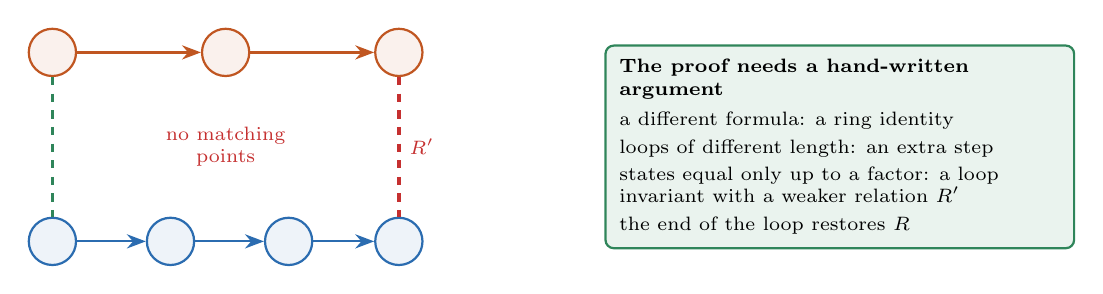
\begin{tikzpicture}[
      st/.style={draw, thick, circle, minimum size=0.6cm, inner sep=0pt, font=\scriptsize}]
    \node[st, draw=realc, fill=realc!8] (x0) at (0, 1.2) {};
    \node[st, draw=refc, fill=refc!8] (y0) at (0, -1.2) {};
    \draw[rel] (x0) -- (y0);
    \foreach \k/\xx in {1/2.2, 2/4.4} {
      \node[st, draw=realc, fill=realc!8] (x\k) at (\xx, 1.2) {};
    }
    \foreach \k/\xx in {1/1.5, 2/3.0, 3/4.4} {
      \node[st, draw=refc, fill=refc!8] (y\k) at (\xx, -1.2) {};
    }
    \draw[flow, realc] (x0) -- (x1);
    \draw[flow, realc] (x1) -- (x2);
    \draw[flow, refc] (y0) -- (y1);
    \draw[flow, refc] (y1) -- (y2);
    \draw[flow, refc] (y2) -- (y3);
    \draw[rel, gapc] (x2) -- node[right, label, text=gapc] {$R'$} (y3);
    \node[label, text=gapc] at (2.2, 0) {no matching\\points};

    \node[proof, text width=5.6cm, align=flush left, font=\scriptsize] at (10.0, 0)
      {\textbf{The proof needs a hand-written argument}\\[3pt]
       a different formula: a ring identity\\[2pt]
       loops of different length: an extra step\\[2pt]
       states equal only up to a factor: a loop invariant with a weaker relation $R'$\\[2pt]
       the end of the loop restores $R$};
  \end{tikzpicture}
  \vspace{1em}

  \begin{itemize}\footnotesize
    \item This part does not come from a tactic.
    \item It is where most of the effort goes.
  \end{itemize}
\end{frame}

% ---------------------------------------------------------------- 9
\begin{frame}{From one unit to full refinement}
  \centering
  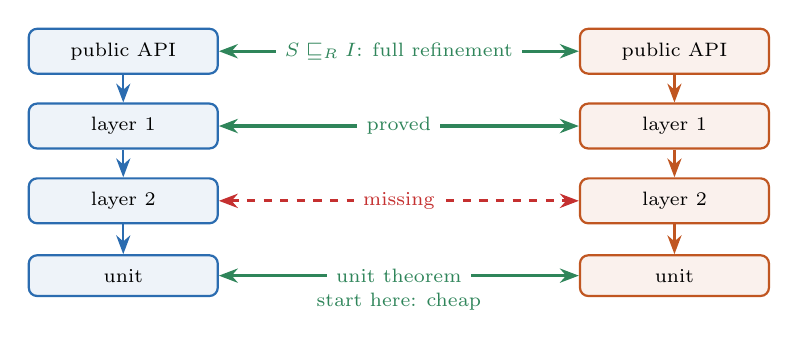
\begin{tikzpicture}[
      lay/.style={box, minimum width=2.4cm, minimum height=0.5cm, font=\scriptsize}]
    \foreach \k/\n/\st in {0/public API/proof, 1/layer 1/proof, 2/layer 2/gap, 3/unit/proof} {
      \node[spec, lay] (s\k) at (0, -\k*0.95) {\n};
      \node[impl, lay] (i\k) at (7, -\k*0.95) {\n};
    }
    \foreach \a/\b in {0/1, 1/2, 2/3} {
      \draw[flow, refc] (s\a) -- (s\b);
      \draw[flow, realc] (i\a) -- (i\b);
    }
    \draw[proved] (s3) -- node[label, fill=paper, text=proofc] {unit theorem} (i3);
    \node[label, text=proofc, below=0.1cm of $(s3)!0.5!(i3)$] {start here: cheap};
    \draw[proved] (s1) -- node[label, fill=paper, text=proofc] {proved} (i1);
    \draw[gapc, very thick, dashed, <->] (s2) -- node[label, fill=paper, text=gapc] {missing} (i2);
    \draw[proved] (s0) -- node[label, fill=paper, text=proofc] {$S \refines_R I$: full refinement} (i0);
  \end{tikzpicture}
  \vspace{0.8em}

  \begin{itemize}\footnotesize
    \item A unit tests the method at a low cost.
    \item Full refinement relates the public API of $I$ to the public API of $S$.
    \item It needs one more result for each layer between the unit and the API.
  \end{itemize}
\end{frame}

% ---------------------------------------------------------------- 10
\begin{frame}{What a theorem trusts}
  \centering
  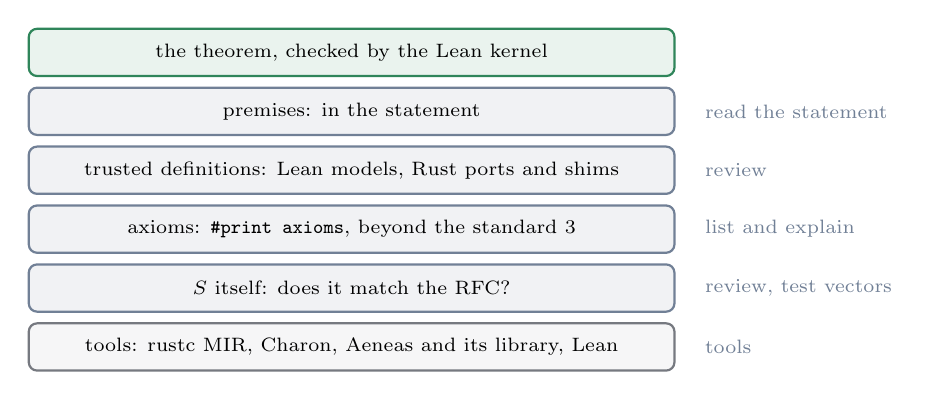
\begin{tikzpicture}[
      layer/.style={box, minimum width=8.2cm, minimum height=0.6cm, font=\scriptsize},
      why/.style={label, text=trustc, anchor=west, align=left}]
    \node[proof, layer] (thm) at (0, 0) {the theorem, checked by the Lean kernel};
    \node[trust, layer, below=0.12cm of thm] (l1) {premises: in the statement};
    \node[trust, layer, below=0.12cm of l1] (l2) {trusted definitions: Lean models, Rust ports and shims};
    \node[trust, layer, below=0.12cm of l2] (l3) {axioms: \code{\#print axioms}, beyond the standard 3};
    \node[trust, layer, below=0.12cm of l3] (l4) {$S$ itself: does it match the RFC?};
    \node[tool, layer, below=0.12cm of l4] (l5) {tools: rustc MIR, Charon, Aeneas and its library, Lean};
    \foreach \n/\t in {l1/read the statement, l2/review, l3/list and explain, l4/{review, test vectors}, l5/tools} {
      \node[why] at ([xshift=0.25cm]\n.east) {\t};
    }
  \end{tikzpicture}
  \vspace{0.6em}

  \begin{itemize}\footnotesize
    \item \code{\#print axioms} does not show trusted definitions. Each study lists them by hand.
    \item Rules: no \code{sorry}, no \code{maxHeartbeats} bump in a proof.
  \end{itemize}
\end{frame}

% ---------------------------------------------------------------- 11
\begin{frame}{Three instances of the method}
  \centering
  \scriptsize
  \renewcommand{\arraystretch}{1.35}
  \begin{tabular}{l l l l}
    & \specside{\textbf{spec $S$}} & \implside{\textbf{impl $I$}} & \textcolor{proofc}{\textbf{proved}} \\
    \hline
    RFC 8439 ChaCha20 & hax-style spec & libcrux HACL & block core (unit) \\
    \textbf{RFC 7748 X25519} & \textbf{hacspec, ported to plain Rust} & \textbf{x25519-dalek} & \textbf{full refinement} \\
    RFC 9180 HPKE & hacspec, behind a shim & hpke-rs & key schedule (unit) \\
  \end{tabular}
  \vspace{1.5em}

  \normalsize
  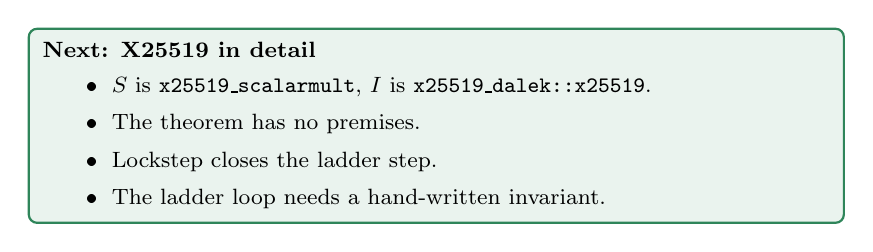
\begin{tikzpicture}
    \node[proof, text width=10cm, align=flush left, font=\footnotesize]
      {\textbf{Next: X25519 in detail}
       \begin{itemize}
         \item $S$ is \code{x25519\_scalarmult}, $I$ is \code{x25519\_dalek::x25519}.
         \item The theorem has no premises.
         \item Lockstep closes the ladder step.
         \item The ladder loop needs a hand-written invariant.
       \end{itemize}};
  \end{tikzpicture}
\end{frame}

\end{document}
